
\section{Optimizing the Basic Approach}
\label{sec:opt}

A major drawback of our \emph{basic} MILP transformation (Section~\ref{sec:sol}) is
that it exhaustively encodes the combination of all tuples in the database and all queries
in the query log.  In this approach, the number of constraints (as well as undetermined variables) 
grows quadratically with respect to the database and the query log.
This increase has a large impact on the running time of the solver, since it needs to find a (near)-optimal 
assignment of all undetermined variables (exponential with the number of undetermined variables).
This is depicted in Figure~\ref{fig:querysize_vs_time}, which increases the query log size over a database of $1000$ tuples.  
The red bars encode the problem using  the \emph{basic} algorithm that parameterizes all queries, while the blue bars show the potential gain of only parameterising the oldest query that we assume is incorrect.
\xlw{At a log size of $80$, the solver for \emph{basic} \textbf{failed} to produce an answer within $1000$ seconds.}
Although MILP solvers exhibit empirical performance variation,
this experiment illustrates the performance limitation of the \emph{basic} approach. 

A second limitation of \emph{basic} is its inability to handle errors in the complaint set.
This is because the \emph{basic} MILP formulation generates hard constraints for all of the database records, thus any error, whether a false negative missing complaint or a false positive incorrect complaint, must be correct.
It may be impossible to find a repair that satisfies this condition and will lead to solver infeasibility errors.


The rest of this section describes three classes of \emph{slicing} optimizations that 
reduce the number of tuples, queries, and attributes that are encoded in the MILP problem. 
The tuple-slicing technique additionally improves the repair accuracy when the complaint set is incomplete. 
We also propose an incremental algorithm that avoids the exponential increase in solver time by only parameterizing a small number of queries at a time---thus limiting
the cost to the left side of Figure~\ref{fig:querysize_vs_time}.







\begin{figure}[t]
    \centering
    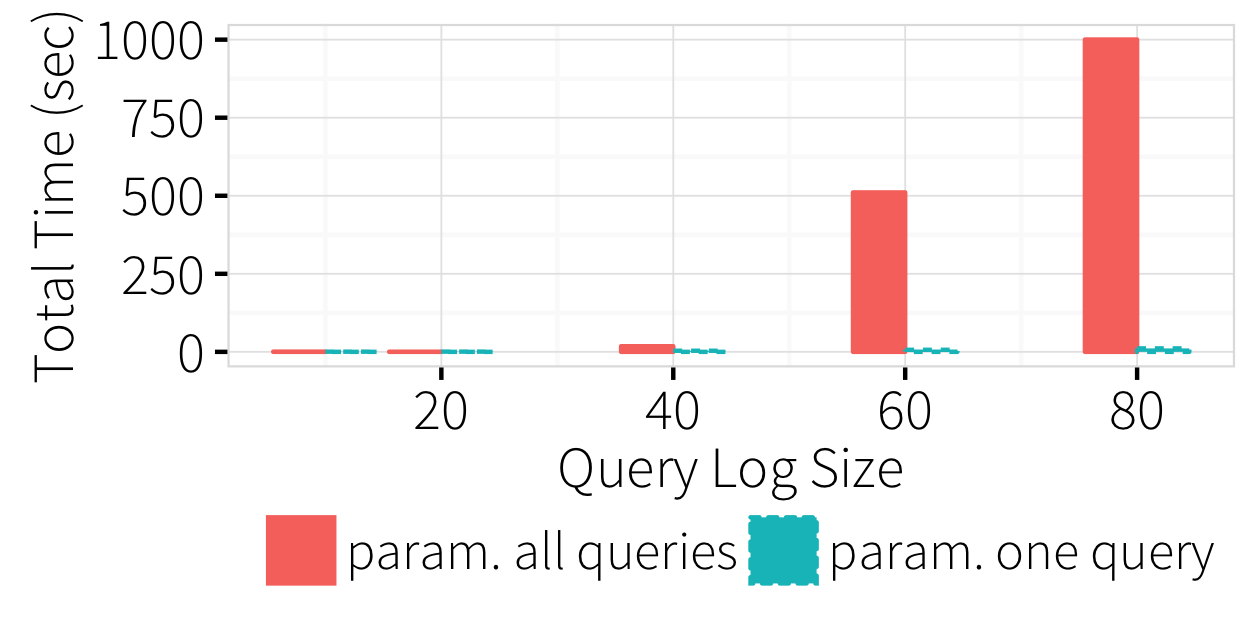
\includegraphics[width=0.35\textwidth]{figures/qsize_time_badscale}
    \vspace*{-0.1in}
    \caption{Log size vs. execution time over 1000 records. }
    \label{fig:querysize_vs_time}
\end{figure}

\begin{figure}[t]
    \centering
    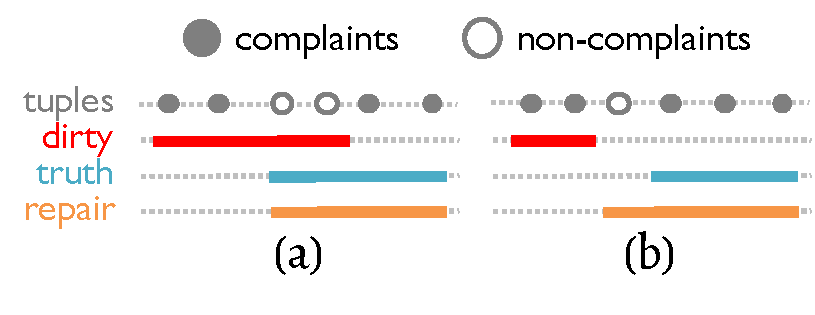
\includegraphics[width=0.35\textwidth]{figures/2nditerationgroups}
    \vspace*{-2mm}
    \caption{
      Graphical depiction of correct (a) and over-generalized (b) repairs.
      Solid and empty circles represent complaint and non-complaint tuples.
      Each thick line represents the interval of query $q$'s range predicate.
      Dirty: incorrect interval in corrupted query;
      truth: correct interval in true query;
      repair: interval returned by the solver.}
    \label{fig:groups}
\end{figure}



\if{0}
linearize whole query log, so cost of adding an additional tuple is very high.
second iteration generally takes ~1 - 10
for large databases knn cost is pretty high: ~

if the solver returns, it is always a super set of the clean range

only tuples modified by the fixed queries
- tuples already in the complaints (correct)
- not in complaints, but any of the originial queries modified it
- not in complaints, but no original queries modified it
\fi



\subsection{Tuple Slicing: Reducing Tuples}
\label{sec:opt:tbsize}


Our first optimization, \emph{tuple-slicing}, applies a two step process to reduce the 
problem size without sacrificing accuracy: it
first aggressively reduces
the problem size by only encoding tuples in the complaint set and then refines the log repair 
through a second but much smaller MILP problem. 

\smallskip
\noindent\textbf{Step 1 (Initial Repair Step):}
The first step of  \emph{tuple slicing} 
aggressively reduces the problem size by only encoding those 
tuples in the complaint set $\mathcal{C}$ (Algorithm~\ref{alg:basic} line $2$
is replaced with \texttt{for each t in $\mathcal{C}$}). 
Each tuple necessitates
the linearization of the entire query log, thus, only encoding the complaint tuples minimizes the 
size of the problem with respect to the relevant tuples. 
This optimization is guaranteed to resolve $\mathcal{C}$, thus depending on the properties of the non-complaint records, it can generate correct repairs
an order of magnitude faster without hurting the accuracy. 
In Figure~\ref{fig:groups}(a),
the solver will guarantee a repair interval that excludes the two left-most complaints, includes the two right-most complaints,
and minimizes the difference between the dirty and repaired intervals (due to the objective function).
This effectively pushes the repair's lower-bound towards that of the dirty interval.
This is a case where such a solution is correct, because the dirty and truth intervals overlap.
Recall that we do not have access to the truth interval, and our goal is to reproduce the truth interval given $\mathcal{C}$ (solid circles) and the corrupted query.

However, this approach can also cause the repair to be a {\it superset} of the truth interval, and affect tuples not part of the complaint set.
Figure~\ref{fig:groups}(b) highlights such a case where the dirty and truth intervals are non-overlapping, and the non-complaint record between them has been incorrectly included in the repair interval---\emph{because the MILP problem did not include the non-complaint.}





\indent In both of these cases, the objective function will ensure that the repair
does not over-generalize the upper bound towards the right because that strictly increases the objective function.
Therefore, our main concern is to refine the repair interval to exclude those non-complaint tuples in case (b).
Note that in the case of incomplete complaint sets, the user may \xlw{choose not to} execute the refinement step if she believes
that the non-complaint records are indeed in error.

\smallskip

\noindent\textbf{Step 2 (Refinement Step):} \looseness -1
Although there are many possible mechanisms to refine the initial repair (e.g., incrementally shrinking
the repaired interval until the non-complaint tuples are all excluded), 
the straightforward approaches are not effective when multiple corrupt 
queries have been repaired because they don't take the query interactions into account.

\looseness -1
Instead, we solve this with a second, significantly smaller, MILP problem.   
Let $\mathcal{Q}^*_{rep}$ be the set of repaired queries from the  initial MILP formulation with tuple slicing;
$\mathcal{NC}$ be the set of non-complaint tuples now matching the repaired \texttt{WHERE} clauses, as in Figure~\ref{fig:groups}(b); and $\mathcal{C}^+ = \mathcal{C} \cup \mathcal{NC}$.
We create a new MILP using $\mathcal{C}^+$ as the complaint set.  
The key is to only parameterize the repaired clauses from Step 1 as constraints with undetermined variables.
The variables for all other tuples and queries are fixed to their assigned values from Step 1.
This \emph{refines} the solutions from the previous step while incorporating knowledge about complaints in $\mathcal{NC}$, 
Finally, we use a new objective function to minimize the number of non-complaint tuples 
$t \in \mathcal{NC}$ that are matched by the solution.


In our experiments, we find that this second MILP iteration adds
minimal overhead ($0.1-0.5\%$) with respect to the initial MILP
problem. 
\xlw{\emph{Tuple-slicing} optimization is primary applied on fixing workload with \textit{range predicates}. The probability of making an incorrect log repair due to tuple-slicing is very low: A failure case only happens when there exists a different set of queries (other than the actual incorrect queries) in the workload that modifies every tuple in the complaint set. In fact, the probability of having such a case in our synthetic datasets is lower than $0.001\%$ but could be higher with less attributes in the database and fewer tuples. For workloads with \textit{point predicates} (a.k.a only a small set of tuples---$1-2$ are updated by each individual query), including most benchmark workloads, with the help of other optimization, queries that might result in a incorrect repair are already pruned ahead , thus applying \emph{tuple-slicing} is guaranteed to be correct.
In summary, \emph{tuple-slicing} is an effective method to improve the performance of the \emph{basic} approach, without compromising, and often improving, repair quality.
}





\if{0}
  \subsubsection{A Naive but Flawed approach}
  \ewu{Better explained as: CPLEX searches through an exponential space of all possible combinations of MILP variables.  In a chunked approach, the solution of each chunk is one out of a potentially arbitrary number of possible solutions, thus it is easy to pick an incorrect one}
  A natural idea to optimize the \emph{basic} approach is 
  to \textbf{chunk the query log} into
  smaller, fixed size pieces and then solve each piece at a time: starting
  from the most recent piece, the system linearizes and parameterizes queries 
  in the current piece and derives a corresponding log repair; 
  it then examines the other pieces iteratively
  in the same way. Since complaints only provides
  true values for the most recent database state, in order to avoid 
  linearizing additional queries, 
  we need to know \textbf{rollback} the true values of tuples 
  until the last query in each query log piece. \\
  However, rollback the database is non-easy. An ideal, precise rollback
  algorithm would generate a set of valid ranges for each attribute of a tuple. 
  But the size of valid ranges also grows exponentially with the number queries
  we want to rollback, which, in turn, could not improve the system performance. 
  On the other hand, an approximate, imprecise 
  rollback algorithm would either make the rest of the problems
  infeasible to solve (only maintain fixed number of valid ranges) 
  or result in deriving 
  incorrect log repairs (maintain the lower 
  bound and upper bound among all valid ranges).
    

  In order to improve the system performance without losing accuracy, we propose
  the following two optimizations: query-slicing optimization 
  based on provenance over queries and
  attribute-slicing optimization based on provenance over 
  attributes. 
\fi





\subsection{Query Slicing: Reducing Queries}
\label{sec:opt:query}

\looseness -1
In practice, many of the queries in the query log could not have affected the \emph{complaint attributes} (defined below). For example, if $q_{N-1}$ and $q_{N}$ 
only read and wrote attribute $A_1$, then they could not have contributed to an error in $A_2$.  
However, if $q_{N}$  wrote $A_2$, then either or both queries may have caused the error. 
In short, if we model a query as a set of attribute read and write operations, those 
not part of the causal read-write chain to the \emph{complaint attributes} can be ignored.
This is the foundation of our \emph{query-slicing} optimization.


\begin{definition} [Complaint Attributes $\mathcal{A}(\mathcal{C})$]
	The set of attributes identified as incorrect in the complaint set.
	\[\mathcal{A}(\mathcal{C}) = \{A_i | t.A_i \neq t^*.A_i, c(t,t^*) \in \mathcal{C}\}\]
\end{definition} 


\begin{definition}[Query dependency \& impact]
    Query $q_i$ has \textbf{direct-impact}, $\mathcal{I}(q_i)$, which is
    the set of attributes updated in its modifier function $\mu_{q_i}$
    (e.g., \texttt{SET} clause). Its \textbf{dependency},
    $\mathcal{P}(q_i)$, is the set of attributes involved in its
    condition function $\sigma_{q_i}$.
    We derive the \textbf{full-impact}, $\mathcal{F}(q_i)$, of a query $q_i$ by propagating its direct impact through subsequent queries in the log (Algorithm~\ref{alg:fullimpact}):
    \[
    \mathcal{F}(q_i)=\mathcal{I}(q_i)\bigcup_{\substack{j=i+1\\ \mathcal{F}(q_{j-1})\cap \mathcal{P}(q_j) \neq \emptyset}}^n \mathcal{F}(q_j)
    \]
\end{definition}






By computing the full-impact of $q$, we can determine the extent that it affects $\mathcal{C}$
based on its overlap with the complaint attributes.
Specifically, 
when $|\mathcal{F}(q) \cap \mathcal{A}(C)|=|\mathcal{A}(C)|$, $q$ may affect all complaint attributes and is a candidate for repair; 
when $0 < |\mathcal{F}(q) \cap \mathcal{A}(C)| < |\mathcal{A}(C)|$, 
$q$ contributed to a subset of the complaint attributes and is a candidate for repair;
when $|\mathcal{F}(q) \cap \mathcal{A}(C)|=0$, $q$ is irrelevant 
and can be ignored during the repair process.
We distinguish between the first and second conditions in the special case where we are repairing a \emph{single} 
corrupted query in the query log.  In this case, only queries in the first conditions are candidates for repair because 
the single query must have caused errors in all of the complaint attributes.  This enables \sys to scale significantly better
for this important problem setting. 
Finally, we use $Rel\mathcal{(Q)}$ to denote the set of relevant
queries that are candidates for repair.

 \xlw{Our \emph{query slicing}
optimization linearizes only the queries in
$Rel\mathcal{(Q)}$, rather than the entire log, resulting in
smaller problems than the \emph{basic} approach \textbf{without any loss of accuracy}.}

\subsection{Attribute Slicing: Reducing Attributes}

In addition to removing irrelevant queries, we additionally avoid encoding irrelevant attributes.
Given $Rel\mathcal{(Q)}$, the relevant attributes can be defined as:
$Rel\mathcal{(A)} = \cup_{q_i \in Rel\mathcal{Q}} (\mathcal{F}(q_i)\cup \mathcal{P}(q_i))$
We propose \emph{attribute slicing} optimization that only encodes constraints for attributes in $Rel\mathcal{(A)}$.
We find that this type of slicing can be effective for wide tables along with queries that focus on a small subset of attributes. 

\xlw{Similar to \emph{query slicing}, \emph{attribute slicing} optimization identifies irrelevant attributes by carefully analyzing incorrect attribute(s)
and their provenance. Thus, applying \emph{attribute slicing} optimization leads to smaller problems and 
\textbf{guarantees the correctness at the same time}. }



\subsection{Incremental Repairs}\label{sec:incremental}



\looseness -1
Even with the slicing optimizations, the number of undetermined variables can remain high, resulting in slow solver runtime.  
The red bars in Figure~\ref{fig:querysize_vs_time} showed the exponential cost of parameterizing the entire query log as compared to only solving for a single query (blue bars).
These results suggest that it is \emph{faster} to run many small MILP problems than a single large one, and motivates our incremental algorithm.

 \looseness -1
Our \emph{$Inc_k$} approach (Algorithm~\ref{alg:incalg}) focuses on the case where there is a single corrupted query to repair.
It does so by linearizing the full query log, including any slicing optimizations, but only parameterizing and repairing a batch of $k$ consecutive queries at a time. 
This procedure first attempts to repair the $k$ most recent queries, and continues to the next $k$ queries if a repair was not generated.
The algorithm internally calls a modified version of the \emph{basic} approach that takes extra parameters $\{q_i, q_{i+k}\}$, only parameterizes those queries, and fixes the values of all other variables.

The incremental approach prioritizes repairs for complaints that are due to more recent corruptions.
Given that the \emph{basic} algorithm simply fails beyond a small log size, we believe this is a natural and pragmatic assumption to use, and results in 
a $10\times$ scalability improvement.
Our experiments further evaluate different batching levels $k$ in the incremental algorithm and show that it is impractical from both a performance and accuracy to have $k > 1$.

\begin{algorithm}[t]
\scriptsize
\caption{$FullImpact:$ Algorithm for finding $\mathcal{F}(q)$.}
\label{alg:fullimpact}
\begin{algorithmic}[2]
\REQUIRE {$\mathcal{Q}$, $q_i$}
\STATE $\mathcal{F}(q_i) \leftarrow \mathcal{I}(q_i)$
\FOR {each $q_j$ in $q_{i+1}, ..., q_{n} \in \mathcal{Q}$}
\IF {$\mathcal{F}(q_i)\cap \mathcal{P}(q_j) \neq \emptyset$}
\STATE $\mathcal{F}(q_i) \leftarrow \mathcal{F}(q_i) \cup \mathcal{F}(q_j)$
\ENDIF
\ENDFOR
\STATE Return $\mathcal{F}(q_i)$
\end{algorithmic}
\end{algorithm}

\begin{algorithm}[t]
\caption{$Inc_k:$ The incremental algorithm. 
}
\scriptsize
\label{alg:incalg}
\begin{algorithmic}[2]
\REQUIRE {$Q, \mathcal{D}_j, \mathcal{D}_n, \mathcal{C}, k$}
\STATE Sort $Q$ from most to least recent
\FOR {each $q_i...q_{i+k} \in Q$}
  \STATE $\mathcal{Q}_{suffix}$ = $\{q_j | j \ge i \}$ 
  \STATE $\mathcal{Q}^*$ $\leftarrow$ $Basic_{params}(\mathcal{Q}_{suffix}, \mathcal{D}_j, \mathcal{D}_n, \mathcal{C}, \{q_i, q_{i+k}\})$
  \IF {$\mathcal{Q}^* \neq \emptyset$}
    \STATE Return $\mathcal{Q}^*$
  \ENDIF
\ENDFOR
\end{algorithmic}
\end{algorithm}




